%This is the first chapter of the dissertation

%The following command starts your chapter. If you want different titles used in your ToC and at the top of the page throughout the chapter, you can specify those values here. Since Columbia doesn't want extra information in the headers and footers, the "Top of Page Title" value won't actually appear.
\pagestyle{plain}

\chapter[Tapless and design agnostic Silicon Photonic spatial switches][Top of Page Title]{Tapless and design agnostic calibration of Silicon Photonic spatial switches}

\textit{\textbf{Abstract - }We leverage the photo-conductance (PC) effect in the doped phase-shifter heaters for both controlling and calibrating the Mach-Zehnder interferometer (MZI) switch elements. Both the steady-state and the transient response are experimentally characterized and compact models for the PC current are developed. Utilizing the PC effect, a topology agnostic algorithm is then outlined. The calibration procedure is experimentally verified against calibration with external photo-detectors using a non-blocking 4$\times$4 Benes switch consisting of six 2$\times$2 MZIs. It is shown that our PC-based approach agrees with the PD-based procedure within less than 2.5\% of difference between the obtained calibrated values. Based on the calibrated PC values, all possible routing configurations are measured for extinction ratio (9.92--21.51dB), insertion loss (0.88--4.59dB), and exhibiting performances far below the 7\% FEC limit (bit error rate of $3.8\times 10^{-3}$) using 25 Gbps 4-level pulse-amplitude-modulation signals (PAM4).}
 sb

\section{Introduction}

The continuous increase in data-center traffic is pushing the bandwidth limits of conventional network interconnects\cite{Cisco_whitePaper}. Low power consumption, small footprint, and CMOS integration compatibility are all characteristics of the Silicon Photonic (SiP) broadband switches that promote them as promising building blocks for realizing new reconfigurable inter- and intra-datacenter optical network architectures\cite{Cheng_DC}. Through steering and readjusting the end-to-end nodes interconnectivity\cite{Shen_ResourceUtilization}, the optical network can be optimized for performance\cite{Wen_DC}, efficient resource allocation\cite{Chen_OSA} and the reduced overall network power by alleviating the need for optical/electrical/optical conversions\cite{Shalf_lowEnergy}. 

The rapid growth and advances in available process development kits (PDK) from silicon photonic foundries \cite{Lim_SIPIntegration} such  as AIM Photonics, IMEC, and IME allow designers to fabricate highly integrated and complicated switch topologies. High performance and impressive port counts such as the 16$\times$16\cite{Lu_16} and 32$\times$32\cite{Lei_32,Celo_HighRadixSwitch_2} have been demonstrated, and a recent record of a 64$\times$64\cite{Chu_64} thermo-optical switch has been accomplished. These broadband switches are constructed by using many cascaded 2$\times$2 Mach-Zehnder interferometer (MZI) elements \cite{dupuis2018impact, cheng2017advanced}. For example, a 32$\times$32 consists of 1024 2$\times$2 elements \cite{Tanizawa_HighRadixSwitch_3} that need to operate simultaneously. However, due to the sensitivity to fabrication variations \cite{Selvaraja_fabircation}, the elements are shifted from the desired state causing, in many cases, a low overall performance of the switch. To achieve an optimal operation in terms of low insertion loss and high extinction ratio per routing configuration, the control signals over the phase-shifter of each 2$\times$2 MZI element must be precisely calibrated for its cross and bar states \cite{Qixiang_smart_routing, huang2018crosstalk}. 

The most common approach to address the calibration requirement is direct integration of photo-detectors (PDs) at the output ports of each MZI element. Although Germanium PDs are compatible with silicon photonics and easy to realize, the integration of hundreds of PDs \cite{Dumais_900PDs} can drastically increase the insertion loss due to the tapping of the propagating signal at each MZI stage in the optical path. In addition, advanced packaging techniques are required to enable simultaneous access to thousands of electrical I/O ports for the calibration process. Solutions with lower number of PDs \cite{Lei_32}, and the use of external PDs \cite{Hung_noPDs} are suggested to reduce loss and design complexity, but at the cost of calibration time. To calibrate each MZI element in the switch, not only multiple paths must be examined, but also sweeping multiple MZIs is required. Moreover, the calibration algorithm must be revised depending on the topology of the switch. Outside of the chip, the use of \textit{external} PDs for calibration can be problematic in deployment since additional calibration might be needed after the installation. The CLIPP \cite{Morichetti_CLIPP} solution does not require tapping of the optical signal, but it still poses packaging challenges and requires complicated electrical circuitry to measure impedances. 

\textbf{Here, we utilize the photo-conductance (PC) effect in silicon doped thermo-optic phase-shifter (waveguide-doped heaters) \cite{Harris_heater} of the MZI elements for calibration and continuous control during the switching operation. It alleviates the electrical packaging challenges and reduces footprint because we utilize the doped heaters for two purposes. As the optical signal propagates through the heater, the interaction between photons and doped silicon generates free electrical carriers. Hence, the doped phase-shifter is also used as an optical power monitor since the optical signal is affecting the conductance of the heater\cite{Dong_PC}. The PC effect is already demonstrated in SiP micro-ring resonator applications \cite{Chrotowski_PC,Gazman_PC,Zhou_PC}, and to the best of our knowledge, this is the first demonstration in MZI based switches.} 

The paper is divided into three sections. First, we present models and experimentally measure the steady state and the transient response of the PC effect. In the second section, based on the operation methodology of the effect, a design agnostic algorithm that supports bi-directional 1$\times$N\cite{Guan_1xN}, N$\times$1 \cite{Horst_mux} and N$\times$N switch topologies is outlined. The calibration algorithm is carried out on six MZI elements constructing a 4$\times$4 Benes switch. Lastly, we validate the calibrated control signals obtained through the PC effect against calibration with external PDs. Based on the calibrated cross and bar states of each MZI element, a look-up table for input-to-output routing configurations is also generated. Each routing configuration is experimentally evaluated for insertion loss, extinction ratio, and bit error rate (BER) of 25 Gbps 4-level pulse amplitude modulation (PAM4) optical signals. 

\begin{figure}[t!]
%trim=left botm right top
\centering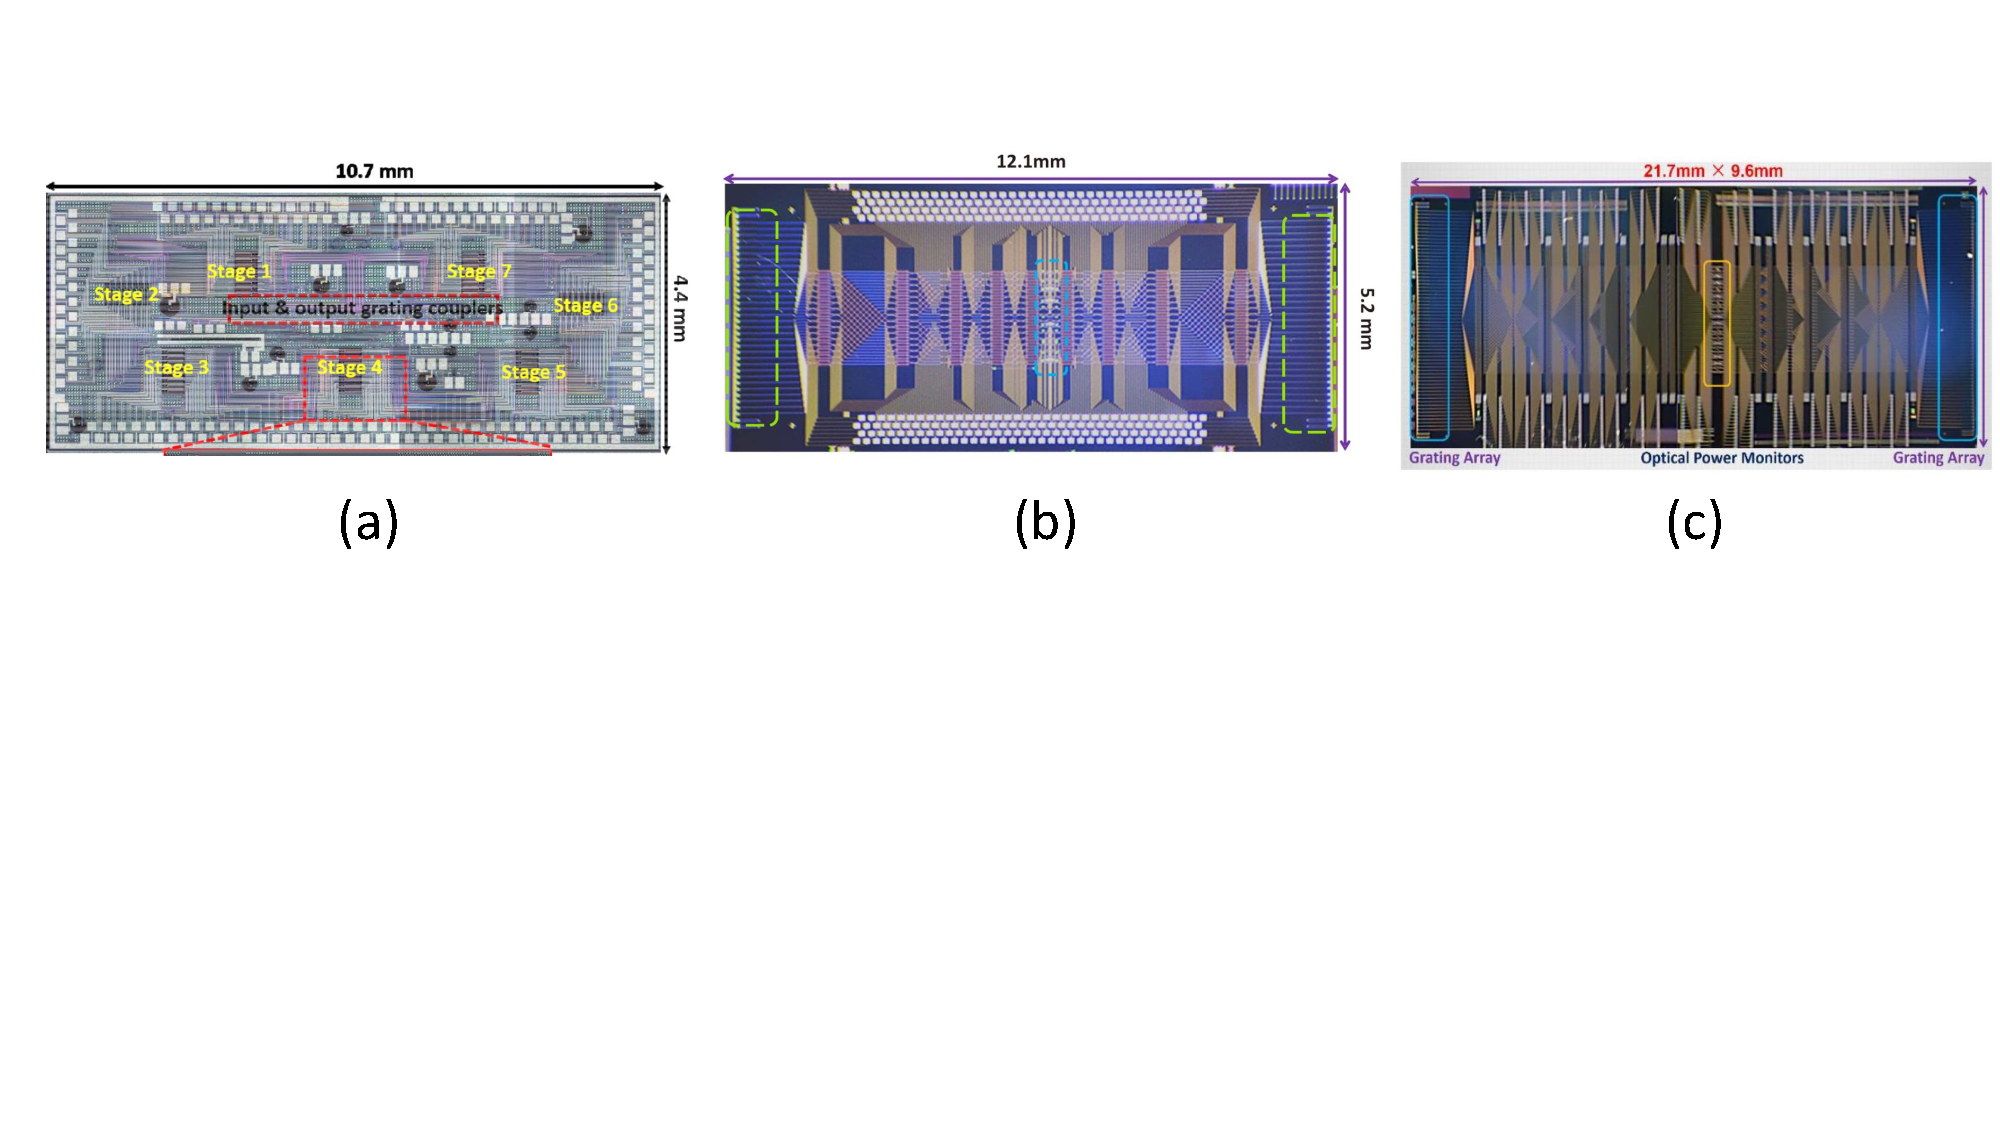
\includegraphics[clip, trim=0cm 8cm 0cm 1cm,width=15cm]{Chapter5/CH_5_fig1.pdf}
\caption{(a) (b) (c)}
\end{figure}






%%%%%%%%%%%%%%%%%%%%%%%%%%  Photo-conductance  %%%%%%%%%%%%%%%%%%%%%%%%%%
\section{Photo-conductance effect}

\begin{figure}[t!]
\centering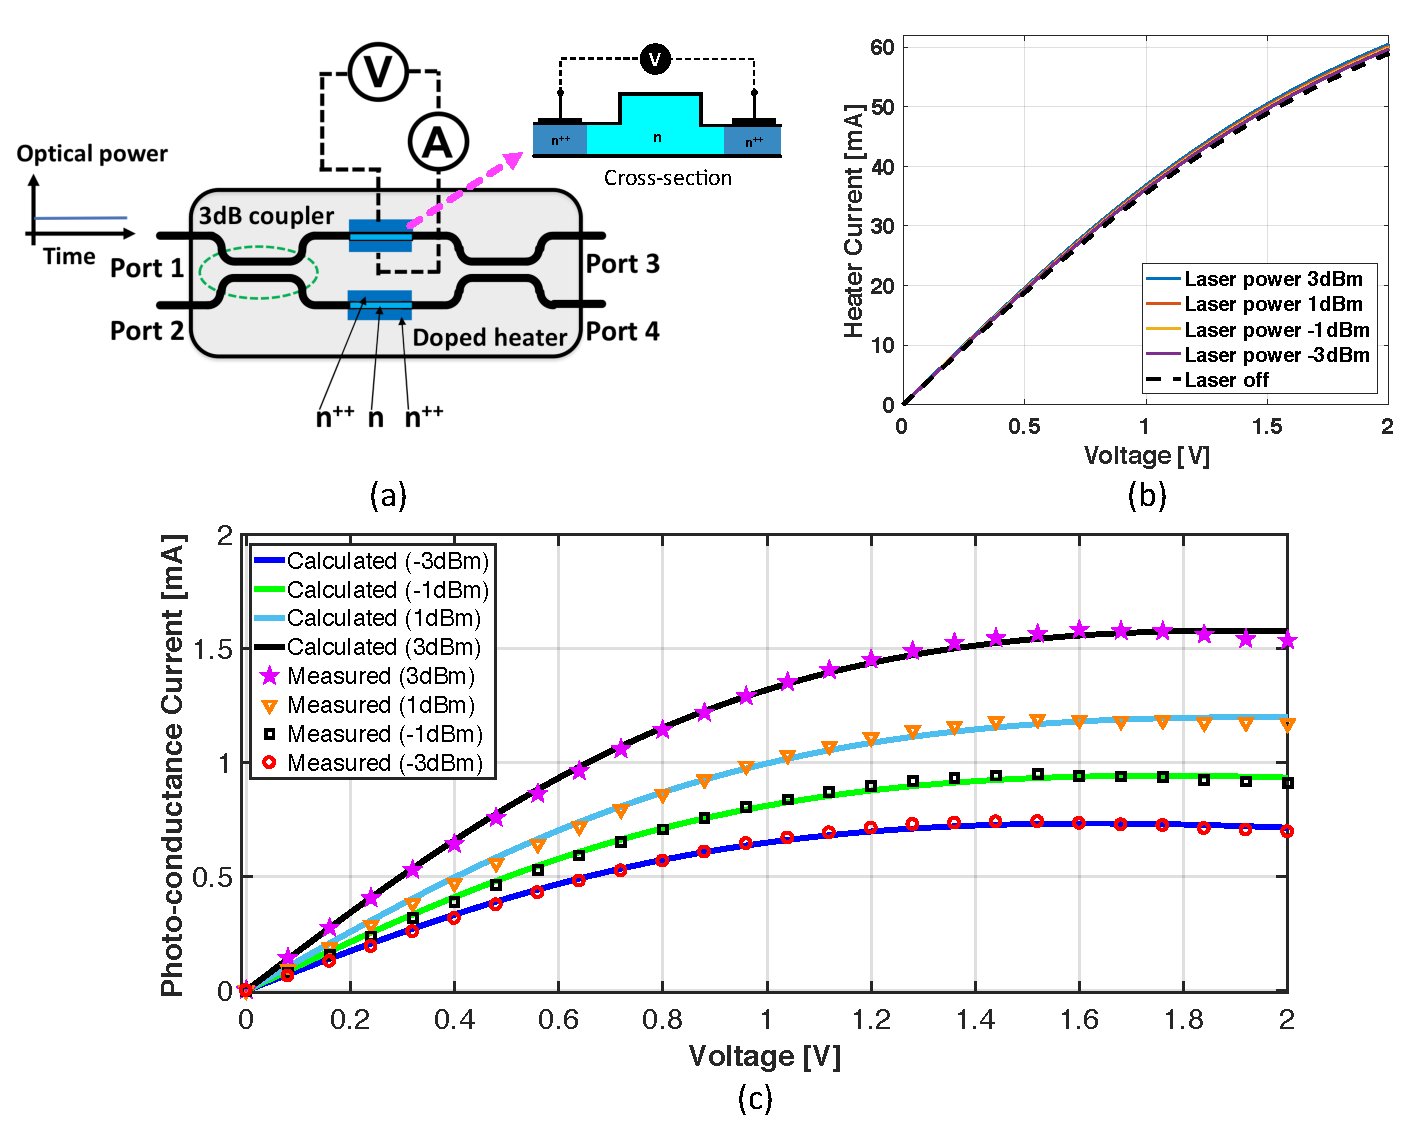
\includegraphics[width=12.5cm]{Chapter5/fig1_MB_v2.pdf}
\caption{(a) Schematic of a 2$\times$2 MZI element with doped-waveguide heater (inset shows the cross-section of the waveguide). An external optical source along with voltage and current meters are used to measure the PC effect. (b) Measured I-V curves of the heater at different input optical power. (c) Calculated (solid) and measured (markers) photo-conductance current , $\Delta I$, at different optical powers and bias voltages.}
\end{figure}

Figure 1(a) shows a schematic of the 2$\times$2 MZI element in our switch equipped with two doped heaters that are used as thermo-optic phase shifters. Each waveguide arm of the MZI is directly doped in a $n^{++}$--$n$--$n^{++}$ configuration \cite{Streshinsky}. To measure the photo-conductance effect, a variable optical power at 1550nm is injected into one of the ports of the MZI element, and a voltage sweep across the heater is performed while recording the heater current. The I-V curve of this doped heater in the absence of optical power follows the nonlinear model of an ohmic resistor due to the self-heating \cite{Bahadori_Self_heating} described by
%
\begin{equation}
\label{eq1}
I(t) = \frac{V(t)}{R_0} \, \frac{2}{1+\sqrt{1+K_v \, V(t)^2}}
\end{equation}
%
where $R_0$ is the linear resistivity at low voltage (or more precisely at low ohmic power) and $K_v$ is the thermal nonlinearity coefficient. The second factor in Eq. (\ref{eq1}) describes the deviation from the linear Ohm's law. The dashed curve in Fig. 1(b) shows the measured I-V response of one of the MZI heating elements in the \textit{absence} of injected optical power. The parameters of the heater are extracted as $R_0 = $  25.824 $\Omega$ and $K_v = $ 0.404 V$^{-2}$. The solid curves in Fig. 1(b) correspond to the measured I-V curves of the heater in the \textit{presence} of optical power inside the waveguide. As it is seen, in the presence of light the I-V curve of the heater moves up slightly showing less resistivity and higher current (\textit{photo-conductance effect}). 

To explain this, we note that the linear and/or nonlinear absorption of light inside the doped waveguide will generate extra electrons and holes that contribute a change to the ohmic conductivity as
%
\begin{equation}\label{eq2}
\sigma = \sigma_0 + \Delta \sigma = \sigma_0 \, (1+K_{p_1} P_\text{wg} + K_{p_2} P_\text{wg}^2)
\end{equation}
%
where $K_{p_1}$ (in units of mW$^{-1}$) is associated with the linear process and $K_{p_2}$ (in units of mW$^{-2}$) is associated with the two-photon absorption\cite{Zhou_PC}, $\sigma_0$ is the original conductivity, and $P_\text{wg}$ is the optical power inside the waveguide (in units of mW). A change in the conductivity subsequently affects the two parameters of the I-V model in Eq. (\ref{eq1}) according to
%
\begin{equation}\label{eq3}
R_0^\prime \approx \frac{R_0}{1+\delta} \quad , \quad K_v^\prime \approx K_v \, (1+\delta)^2 \approx K_v \, (1+2\delta) .
\end{equation}
%
where $\delta = K_{p_1} P_\text{wg} + K_{p_2} P_\text{wg}^2$ is the relative change in the ohmic conductivity of the heater (see Appendix I in \cite{Bahadori_Self_heating}). This is observed in Fig. 1(b) with the slight increase in the I-V curve of the heater for increased input optical power. In table \ref{table1}, $R_0^\prime$, and $K_v^\prime$ are extracted for all the five cases in Fig. 2(b) using a nonlinear least squares fitting. The value of parameter $\delta$ is then evaluated for each case using an average value of
%
\begin{equation}
%\delta \approx \sqrt{\frac{K_v^\prime}{K_v} \times \frac{R_0^\prime}{R_0}} -1 \, .
\delta \approx \frac{1}{2}\left[\sqrt{\frac{K_v^\prime}{K_v}} + \frac{R_0}{R_0^\prime}\right] -1
\end{equation}
%
As expected, increasing the input optical power will lead to an increase in $K_v$ (9.4\%) and $\delta$, while $R_0$ shows a decreasing trend (4.3\%). The value of $R_0 \times K_v$ also exhibits a steady increase of 4.6\% which is close to the decrease rate in $R_0$ and is in  good agreement with Eq. (\ref{eq3}).

By substituting the parameters of Eq. (\ref{eq3}) in the I-V equation Eq. (\ref{eq1}) the following result for the photo-conductance current $\Delta I$ = $I(P_{wg}) - I(P=0)$ is obtained:
%
\begin{equation}\label{eq4}
\Delta I = 2V \left[\frac{1}{R_0^\prime} \, \frac{1}{1+\sqrt{1+K_v^\prime \, V^2}} - \frac{1}{R_0} \, \frac{1}{1+\sqrt{1+K_v \, V^2}} \right] .
\end{equation}
%
Note that even if $K_v \rightarrow 0$, the photo-conductance current can exist, however, the $\Delta I-V$ curve will be linear. The deviation from a linear characteristic is mainly due to the $K_v$ factors that represent the thermal self-heating of the waveguide.
Figure 1(c) plots the theoretically calculated and experimentally measured photo-conductance current, $\Delta I$, indicating a good agreement. A clear dependence on the optical power at any bias voltage (higher optical power results in higher current) is observed, which can be used as a means to monitor the optical power inside each arm of the MZI by sensing the amount of the extra current.


\begin{table}[t] 
\footnotesize
\centering
\caption{Extracted heater parameters in the absence and presence of optical power inside the waveguide.}
\begin{tabular}{lccccc|c}
\hline
\textbf{P$_\text{laser}$ (dBm)} & \textbf{$-\infty$} & \textbf{-3} & \textbf{-1} & \textbf{1} & \textbf{3} & \textbf{Trend} \\ \midrule
\textbf{$R_0 \, (\Omega)$} & 25.824 & 25.2513 & 25.1244 & 24.9837 & 24.7188 & 4.3\% decrease \\ \hdashline
\textbf{$K_v \, (\textrm{V}^{-2})$} & 0.404 & 0.4264 & 0.4294 & 0.4321 & 0.4418 & 9.4\% increase \\ \hdashline
\textbf{$R_0 \times K_v$} & 10.4329 & 10.7672 & 10.7884 & 10.7955 & 10.92 & 4.6\% increase \\  \hdashline
\textbf{$\delta$} & 0 & 0.025 & 0.03 & 0.034 & 0.045 & increase \\ \bottomrule
\end{tabular}
\label{table1}
\end{table}




\subsection{Response time of the photo conductance effect}

\begin{figure}[b]
\vspace{-4mm}
\centering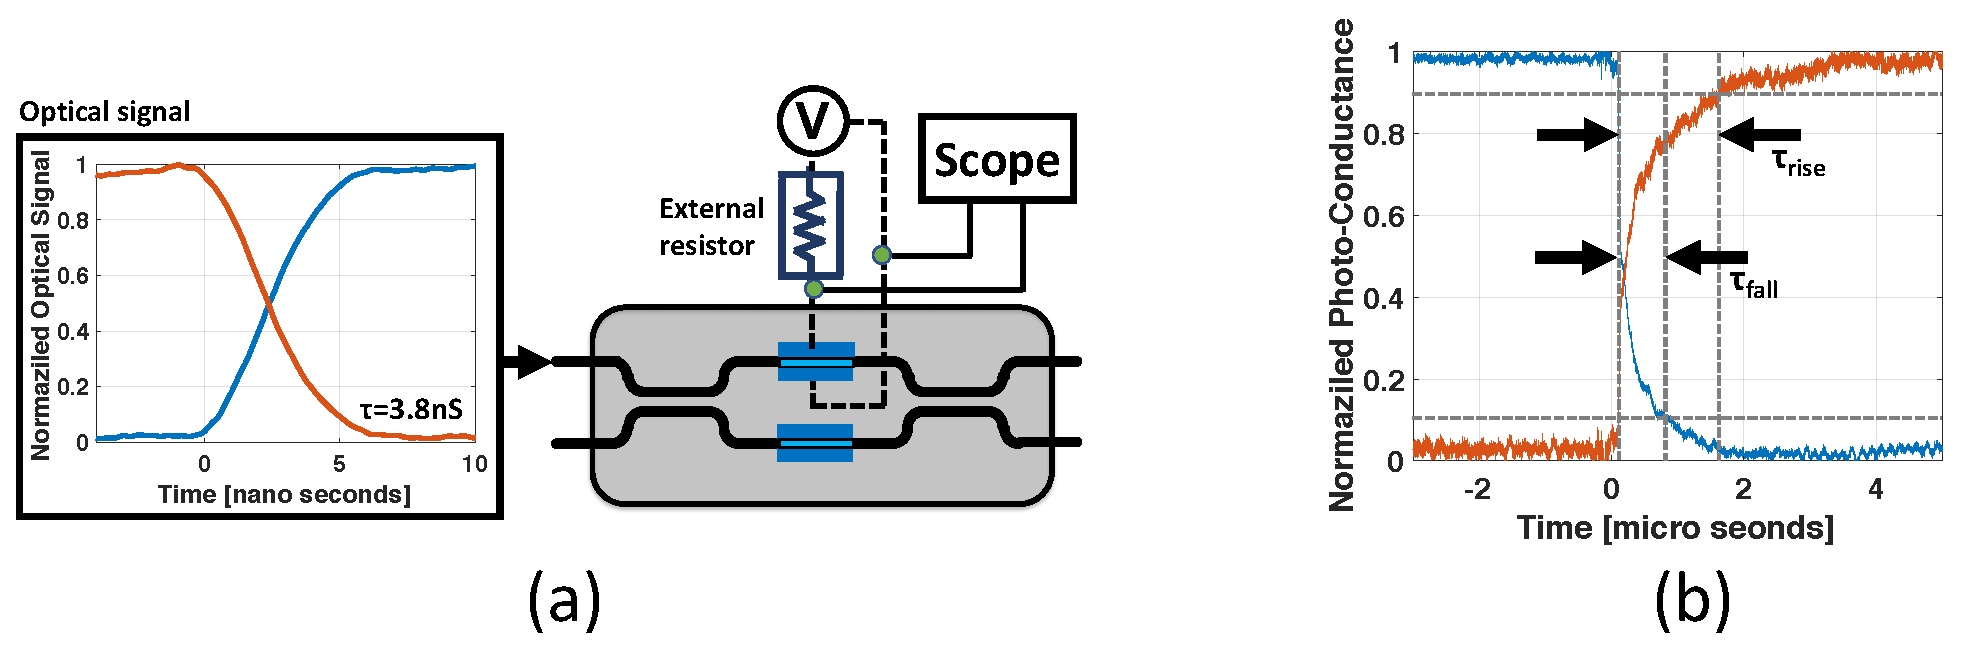
\includegraphics[scale=0.4]{Chapter5/fig2_trans_3}
\caption{(a) Schematic of the photo-conductance transient measurement. (b) Transient response of an optical step function signal. The blue curve corresponds to the rising edge of optical power and the red corresponds to the falling edge of optical power.}

\end{figure}

The transient response time of the PC effect is essential for the calibration procedure and hardware development since it determines the necessary wait time for the effect to reach the steady state. 

As illustrated in Fig. 2(a), a continuous square optical signal is injected into one of the MZI element ports while a steady bias voltage is applied through an external serial resistor. As shown here, the rise and fall times of input optical signal is measured to be 3.8 nsec. 
%
A scope is connected in parallel to the doped heater of the MZI to measure the voltage drop as a function of time. Due to the PC effect, as the optical power increases the resistivity value of the doped heater decreases and the voltage also decreases. Figure 2(b) shows a normalized measured transient response (read out voltage across the heater) for both the rising and falling edges of the optical signal. The blue curve (falling edge of voltage) corresponds to the low-to-high optical step function (rising edge of the optical power)  with a rise-time response $\uptau_{rise}$ (10\% to 90\% change) of 0.7 $\mu$sec and the red curve (rising edge of voltage) corresponds to the high-to-low optical step function (falling edge of the optical power) with a fall-time response $\uptau_{fall}$ (90\% to 10\% change) of 1.5 $\mu$sec. Clearly, these rise and fall times are much larger than the rise and fall times of the input optical pulses. These results correspond to a frequency bandwidth of $\sim100$ KHz which has also been reported in\cite{Dong_PC}.














%%%%%%%%%%%%%%%%%%%%%%%%%  Calibration algorithm  %%%%%%%%%%%%%%%%%%%%%%%%%



\section{Photo-conductance calibration}

\subsection{Calibration algorithm}
The topology-agnostic calibration algorithm based on the PC effect is outlined in the psuedo-code of Fig. 3(a). The algorithm iterates through every MZI element in the switch topology (1$\times$N, N$\times$1 and N$\times$N) to find the necessary control bias voltages over the phase-shifters to set it for the CROSS or BAR states. Figure 3(b) illustrates a generic topology of cascaded MZI elements: ``A'', ``B'', ``C'' and ``D'' in a switch design. The algorithm performs the calibration in an iterative manner starting with the MZI elements connected to the optical I/O interface. The algorithm first establishes an optical path to the MZI element under calibration. In the example of Fig. 3(b), if MZI ``A" is connected directly to the optical I/O port of the switch, no further action is required because the optical path is pre-established. Whereas for the inner MZI elements in the switch topology, the optical path is established based on the previously calibrated MZIs.


\begin{figure}[ht!]
\centering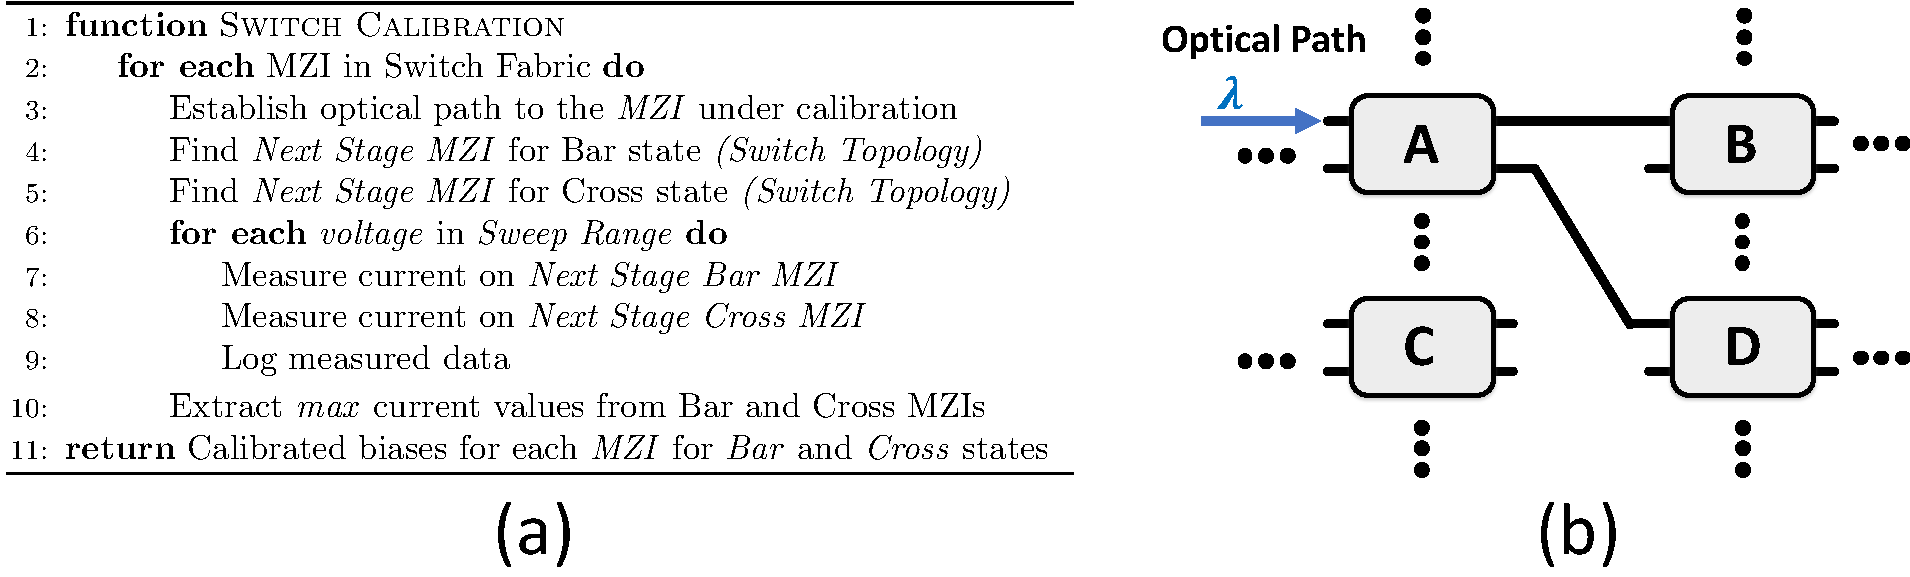
\includegraphics[width=13.5cm]{Chapter5/fig3_alg}
\caption{(a) Psuedo-code of the calibration algorithm. (b) A generic switch section topology of cascaded MZIs. }
\end{figure}

In the next step, the algorithm identifies the two MZIs optically wired to the MZI under calibration within the optical path. In the example of Fig. 3(b),  MZI ``B" and ``D" are used to monitor the PC excess current in the calibration procedure of MZI ``A". In this configuration and based on the optical path, when the maximum optical power is propagating to MZI ``B", MZI ``A" is in BAR state, and when the maximum optical power is propagating to MZI ``D", MZI ``A" is in the CROSS state. To identify these states, the control voltage is swept over MZI ``A" while 1V over the doped-heaters is applied on the MZI ``B" and ``D" and the source's current is logged. Due to the PC effect, the current change is directly related to the optical power. The bias points of MZI ``A" at the maximum current values are measured from the monitoring MZIs ``B"  and ``D" indicating the calibrated values for the BAR and CROSS states, respectively. At the end of the procedure, the algorithm returns a look-up table with each element's associated CROSS and BAR control biases.  

\subsection{Calibration of a 4$\times$4 switch}
The calibration based on the PC effect is performed on a SiP non-blocking 4$\times$4 switch illustrated in the Fig. 4(a) (the layout is outlined in \cite{Qixiang_smart_routing}). The switch consists of eight bi-directional optical I/O ports where the left-sided are denoted as inputs and the right-sided as outputs, and six optically wired 2$\times$2 MZI elements. Each MZI is equipped with two doped heaters to control the state of the switch in a push-pull approach \cite{Yishen_Push_Pull}, however, here we use only the top arm doped heater in the calibration process. 

\begin{figure}[t!]
\centering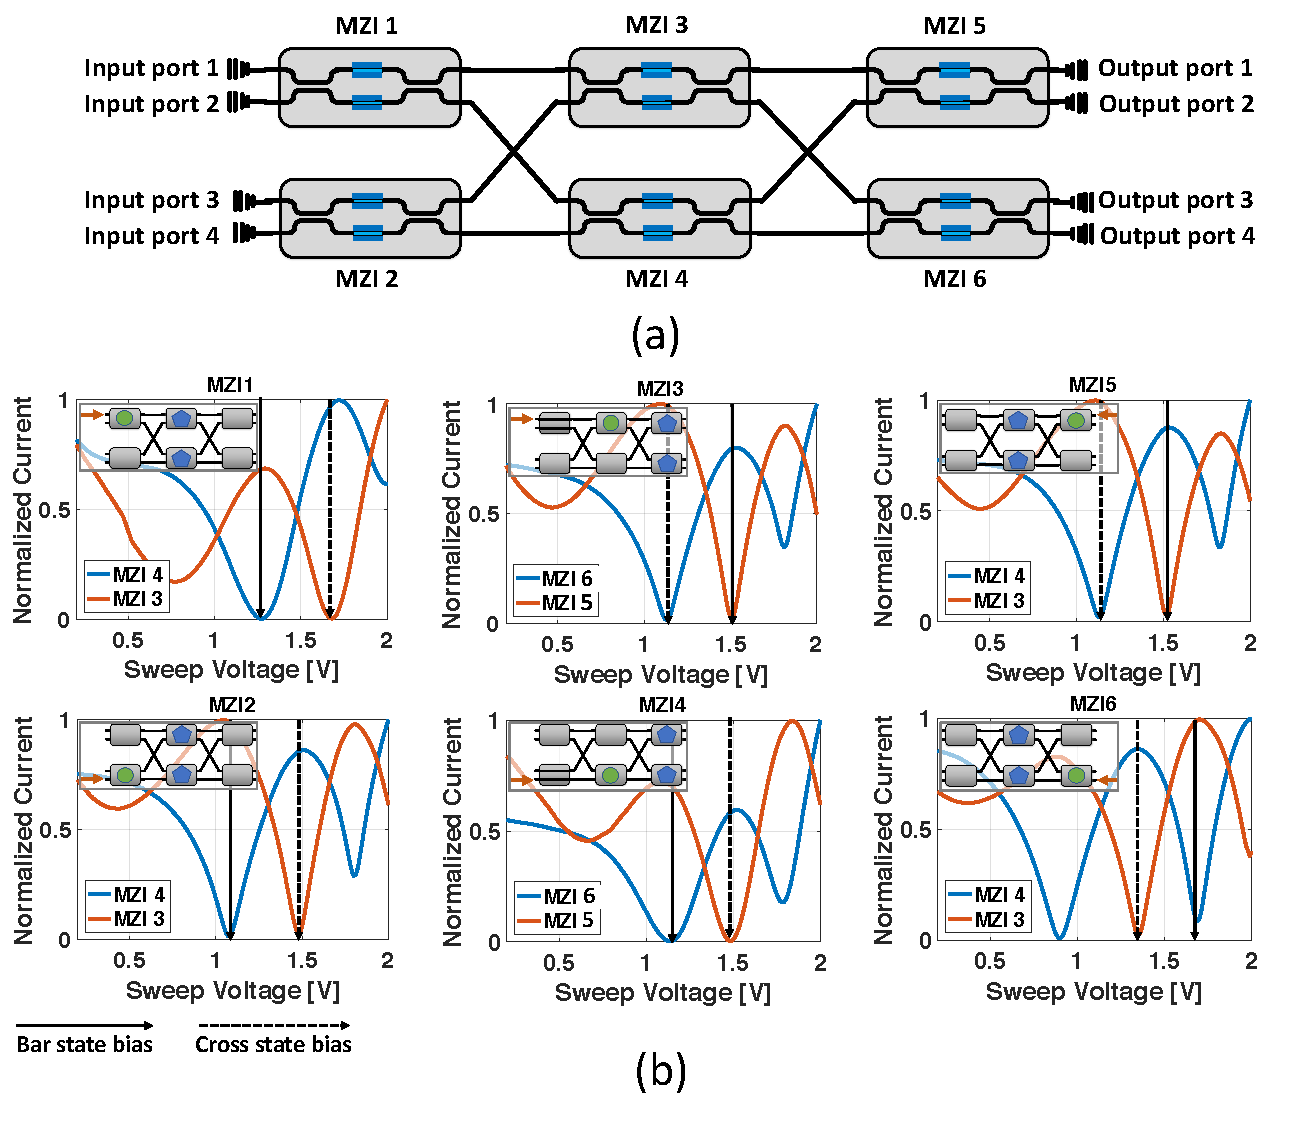
\includegraphics[width=13.5cm]{Chapter5/fig4_PC_switch_2}
\vspace{-4mm}
\caption{(a) Schematic of a the 4$\times$4 switch consisting of six MZI elements. (b) Measured PC calibration results of six MZI elements in 4$\times$4 non-blocking topology. Each plot corresponds to a single MZI element and the curves are measured currents of the proceeding MZI elements with optical path. The insets show the switch topology with the green circles corresponding to the calibrated element and the two blue pentagon shapes corresponds to the monitored elements.}
\end{figure}

The measured calibration results of each MZI element in the switch are shown in Fig. 4(b). The calibration is performed sequentially from MZI1-MZI6. The curves in the plots represent the normalized sourced current from the monitoring MZIs while 1V bias is applied and sweeping the MZI under calibration between 0-2V. The plots' insets represent the calibration setups during the algorithm process where the orange arrow is the optical source (1550nm) input, the green circle is the MZI under calibration and the two blue pentagons shapes represent the monitoring MZIs. Based on the algorithm procedure, the first MZIs to be calibrated are the ones connected to the optical I/O of the switch. Starting from MZI1, the optical signal is coupled through the top input of the 2$\times$2 element, therefore, maximum sourced current on MZI3 indicates the BAR state and the maximum current at MZI4 (or minimum at MZI3) indicates the CROSS state for MZI1. Considering the optical coupling port in the calibration result of MZI2, maximum current at MZI3 indicates the CROSS state for MZI2 while maximum current at MZI4 indicates BAR state for MZI2. 


The calibration of the inner MZIs (3 and 4), requires information of the previously calibrated elements. Continuing with MZI3, the algorithm sets the optical path by applying appropriate control voltage for a BAR state on MZI1 (inset of Fig. 4(b) - MZI3), and utilizing MZI5 and MZI6 as monitoring elements. Similarly, the optical path to MZI4 was set by biasing MZI2 to the BAR state. Lastly, the calibration of MZI5 and MZI6 is implemented by coupling the optical signal through the output ports while MZI3 and MZI4 are used as the monitoring elements.  




The vertical solid and dashed arrows in Fig. 4(b) indicate the calibrated control voltages to set each MZI element to the BAR and CROSS states, respectively. In the next section, the calibrated results are used to control the 4$\times$4 switch, and all possible routing configurations are evaluated for insertion loss, extinction ratio and the quality of optical data switching performances. 


Note that a change in the input optical power will modify the bias voltages necessary to put a 2$\times$2 switch element in the Bar or Cross state. However, by combining Eq. \mbox{(\ref{eq1})} through Eq. \mbox{(\ref{eq3})} it is possible to add a corrective term to the bias voltages after the initial characterization of the heaters is done. The variable that remains unchanged is the required change of temperature of waveguide and it is linearly proportional to the required ohmic power. Therefore, the bias voltages measured at a particular optical power will have to decrease if the optical power is increased and vice versa.



% Please add the following required packages to your document preamble:
% \usepackage[table,xcdraw]{xcolor}
% If you use beamer only pass "xcolor=table" option, i.e. \documentclass[xcolor=table]{beamer}
% \begin{table}[ht]
% \footnotesize
% \centering
% \begin{tabular}{l|c|c|}
% \cline{2-3}
% & \multicolumn{1}{l|}{\textbf{Bar state [V]} } & \multicolumn{1}{l|}{\textbf{Cross state [V]} } \\ \hline
% \rowcolor[HTML]{C0C0C0} 
% \multicolumn{1}{|l|}{\cellcolor[HTML]{C0C0C0}\textbf{MZI 1}} & 1.25 & 1.64 \\ \hline
% \multicolumn{1}{|l|}{\textbf{MZI 2}}                         & 1.09 & 1.51 \\ \hline
% \rowcolor[HTML]{C0C0C0} 
% \multicolumn{1}{|l|}{\cellcolor[HTML]{C0C0C0}\textbf{MZI 3}} & 1.49 & 1.10 \\ \hline
% \multicolumn{1}{|l|}{MZI 4}                                  & 1.13 & 1.47 \\ \hline
% \rowcolor[HTML]{C0C0C0} 
% \multicolumn{1}{|l|}{\cellcolor[HTML]{C0C0C0}\textbf{MZI 5}}          & 1.55 & 1.18 \\ \hline
% \multicolumn{1}{|l|}{\textbf{MZI 6}}                                & 1.74 & 1.40 \\ \hline
% \end{tabular}
% \caption{Extracted calibrated biases of each MZI element in the 4x4 switch for cross and bar states}
% \end{table}


% \begin{figure}[ht!]
% \centering\includegraphics[width=3.5cm]{fig5_biases}
% \caption{Extracted calibrated biases of each MZI element in the 4x4 switch for cross and bar states}
% \end{figure}





%%%%%%%%%%%%%%%%%%%%%%%%%  Discussion  %%%%%%%%%%%%%%%%%%%%%%%%%
\section{Calibration evaluation}
\subsection{Experimental setup}



\begin{figure}[t]
\centering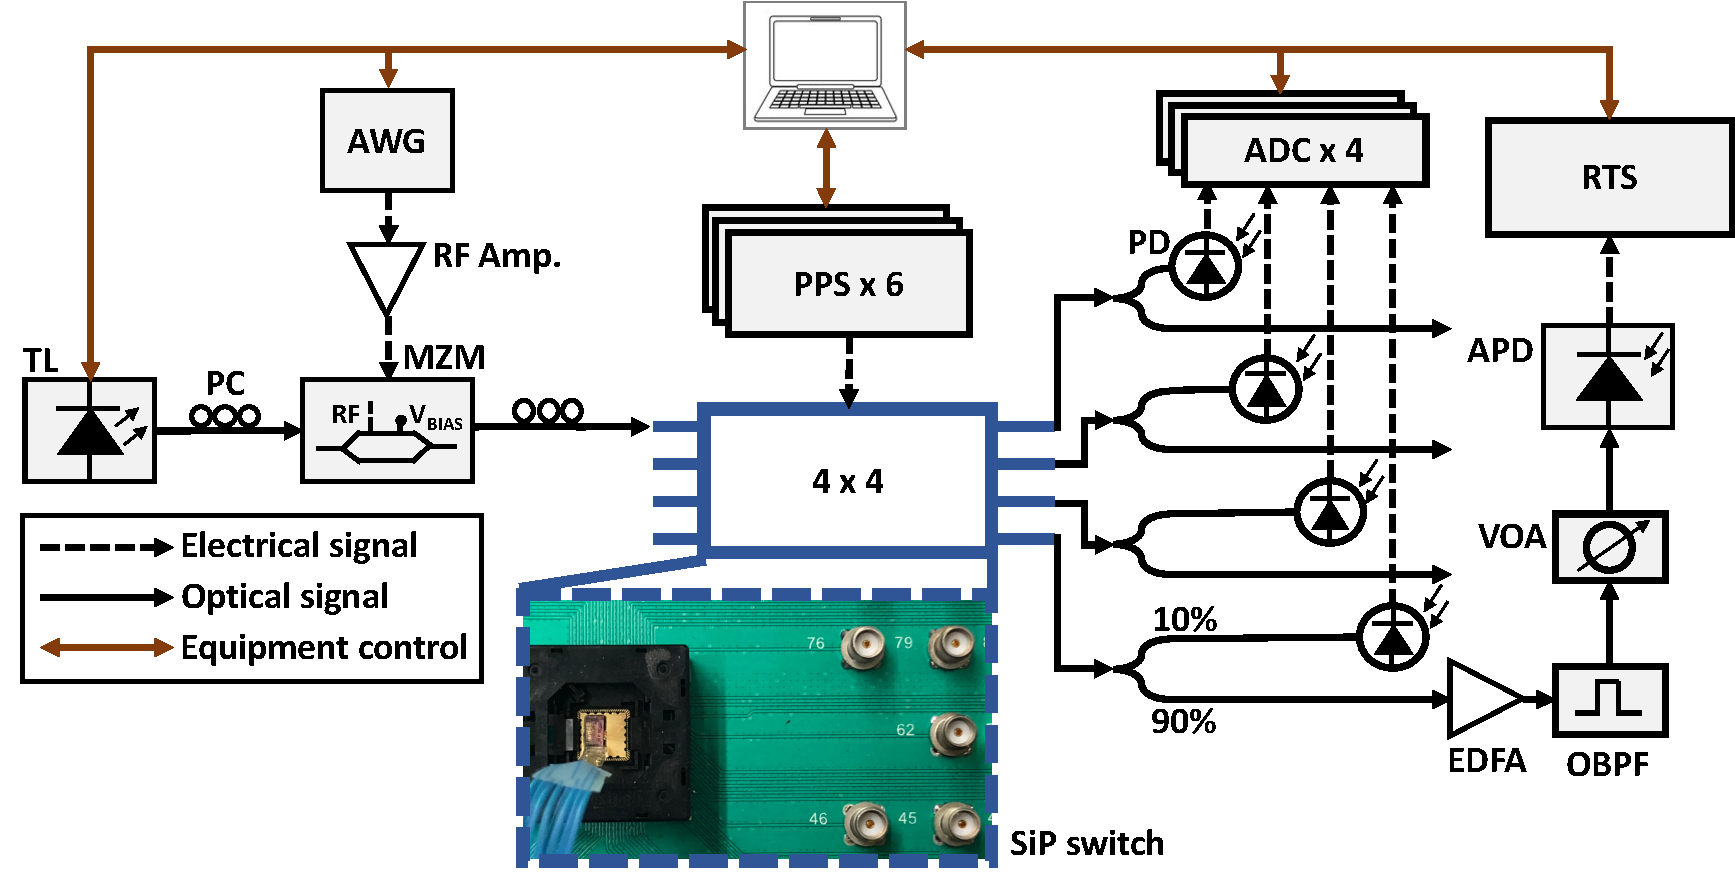
\includegraphics[width=13cm]{Chapter5/fig6_experimental}
\caption{\label{fig:setup}Schematic of the experimental setup. The setup consists of a packaged SiP switch, central control computer and the following equipment: control Arbitrary Waveform Generator (AWG), Tunable Laser (TL), Polarization Controller (PC), Mach-Zehnder Modulator (MZM), Precise Power Supply (PPS), Photo-detector (PD), Analog-to-Digital Converter (ADC), Erbium Doped Fiber Amplifier (EDFA), Optical Bandpass Filter (OBPF), Variable Optical Attenuator (VOA), Avalanche Photo-diode (APD) and Real-Time Scope (RTS).}

\end{figure}





The experimental setup is developed to verify the results of the PC calibration against calibration using external PDs, as well as to evaluate the performance of the switch as a system. Fig. \ref{fig:setup} shows a schematic of the experimental setup with the SiP 4$\times$4 switch in the center. The switch is wire-bonded on a chip carrier and mounted on a breakout printed-circuit-board to allow convenient access to the doped phase shifters of the MZI elements. An array of eight fibers is aligned and glued on top of grating couplers for optical I/O interface. 

The PC calibration algorithm is implemented in the central control computer in Python and serially interfaced to six PPSs (Keithley 2280). The PPSs are used to supply control voltages and to allow the measurement of the PC current. An optical signal (1550nm) is generated using a programmable TL and coupled into the SiP switch through a polarization controller. To validate the calibrated procedure against calibration with external PDs and to measure the steady-state insertion loss and extinction ratios, the four optical output ports are coupled to an optical splitter with 10\% of the light directed to MHz range PDs (Thorlabs PDA20CS) in each case. The PDs are connected to four ADCs (NiDAQ 6363) for power readout and results plotting.

The optical transmission is carried out by programming an AWG (Keysight M8195A) to generate 4-level pulse amplitude signals (PAM4) at 12.5 Gbaud (25 Gbps). The electrical PAM signal is amplified and then used to modulate the light from the TL using a Mach-Zehnder Modulator (MZM). Digital processing (timing deskew, resampling, adaptive equalization, matched filtering, amplitude offset compensation) and bit-error rate (BER) calculations, are performed off-line using MATLAB from the received RTS (Tektronix MSO71254C) signal. At each output port 90\% of the signal is connected to an EDFA to compensate for 10dB fiber to chip coupling loss (~5dB per grating coupler). The OBPF is used to filter the amplified spontaneous emission (ASE) noise associated with the EDFA, and the VOA used to set the optical signal falling on the APD at -5dBm.


% * <browninc@tcd.ie> 2018-09-21T15:53:06.945Z:
% 
% > (PC)
% PC definied both as photo conductance and pol. controller
% 
% ^ <browninc@tcd.ie> 2018-09-21T15:53:51.480Z.


\subsection{Calibration with external photo-detectors}

\begin{figure}[t]
\centering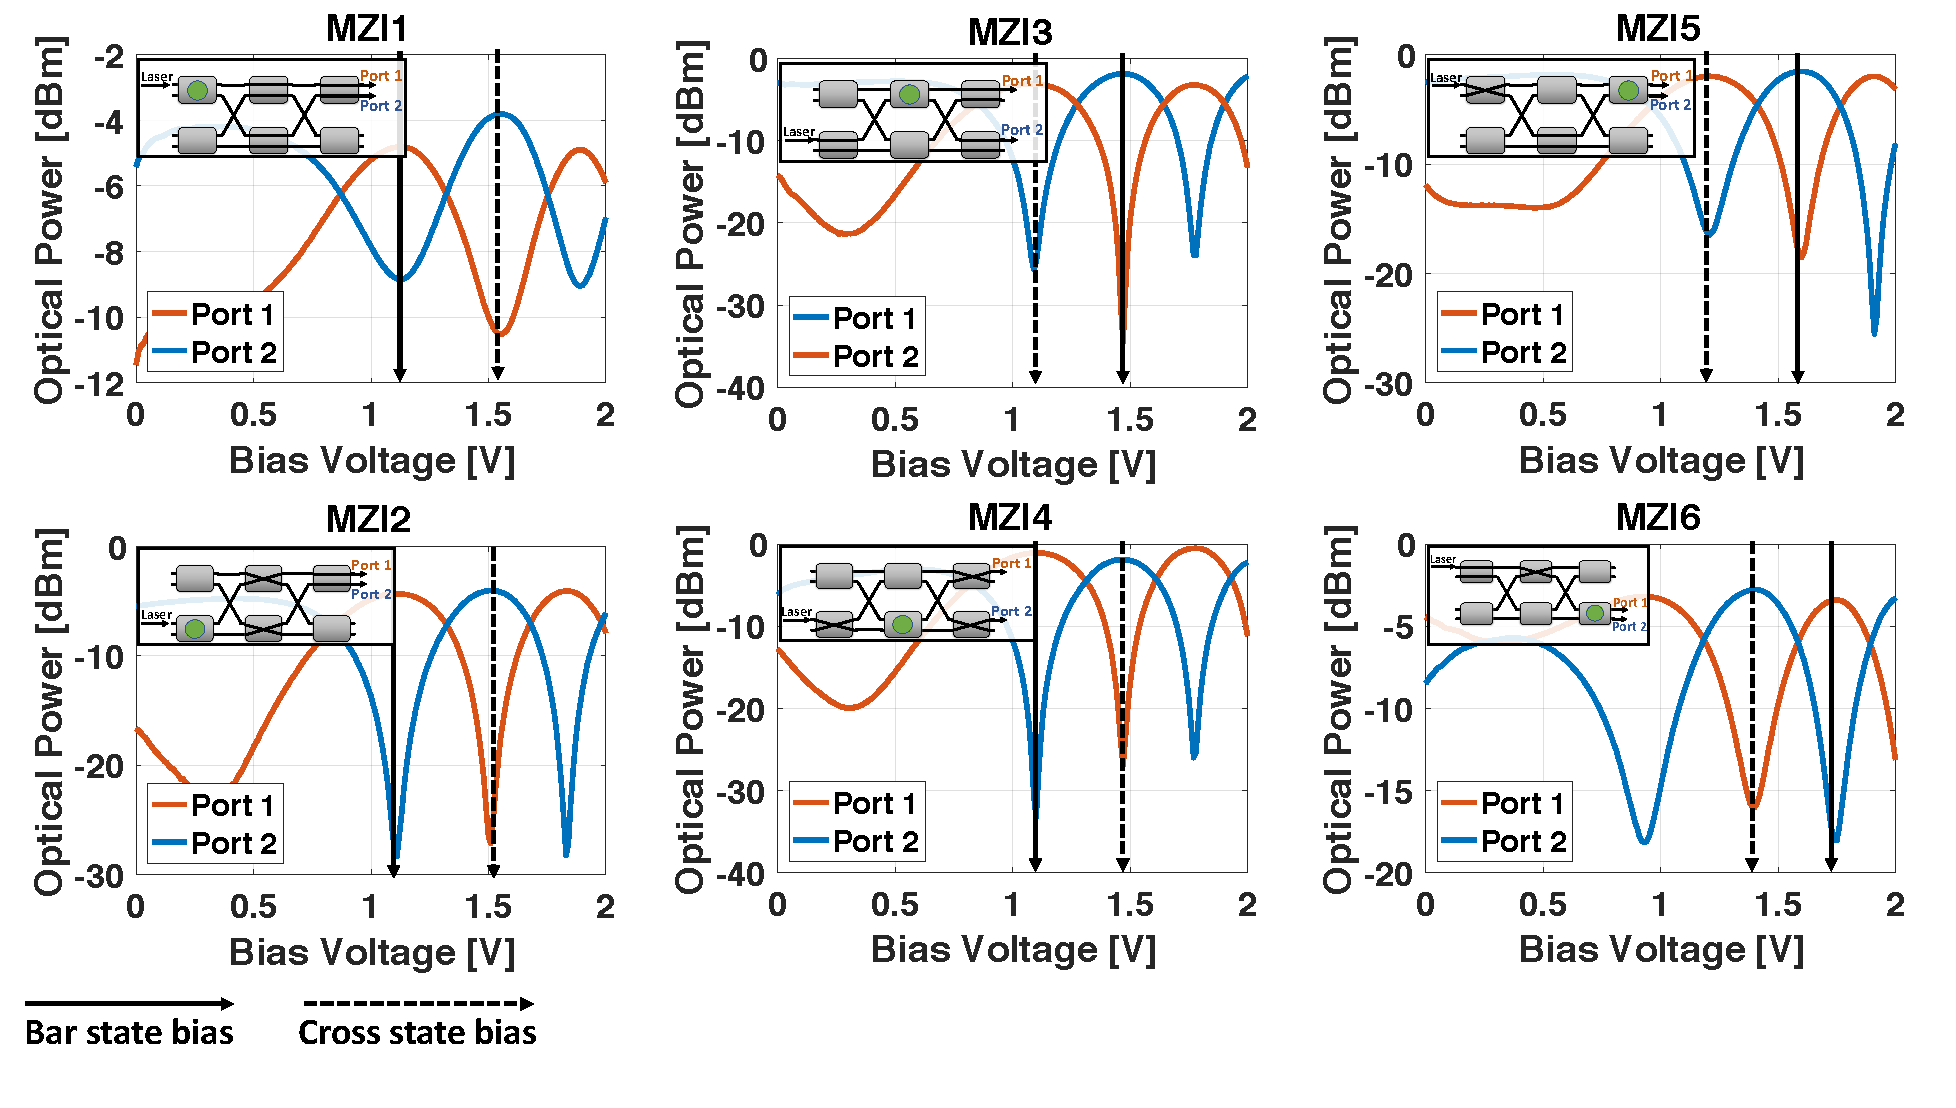
\includegraphics[width=13cm]{Chapter5/fig7_PD_charac}
\caption{Calibration of the six elements in the 4$\times$4 switch using external PDs. The insets show the MZI under calibration (marked with a green circle) and the states of supporting elements as well as the input and output optical ports.}
\end{figure}

To validate the obtained control biases for the CROSS and BAR states of each MZI element in the switch, a calibration with external PDs is performed. An optical path to the MZI under calibration and the external PDs is established using the pre-calibrated values from the PC algorithm. The plots in Fig. 6 show the measured optical power obtained from the PDs and read from the ADCs while several MZI elements set to either CROSS or BAR state and the MZI under calibration is swept again from 0-2V using the PPS. The insets of the Fig. 6 show the optical configuration of the switch during the specific MZI calibration, with the MZI marked with green circles indicate the MZI under calibration. In the case of MZI1, the optical signal is coupled from input port 1 and MZI3-5 are all set to the BAR state to guide the signal to the output ports. In this optical path configuration, MZI1 is in the BAR state when maximum optical power observed at port 1  and in the CROSS state when maximum optical power is measured at port 2. In the calibration process of MZI6, for example, MZI1 is set to BAR and MZI3 is in CROSS. In this configuration, the optical signal is guided directly to MZI6, and based on the input port to the element, maximum received power at port 1 corresponds to the BAR state and port 2 to the CROSS state. The solid and the dashed vertical arrows in Fig. 6 indicate the BAR and CROSS state of each MZI element. 


% \begin{table}[h]
% \footnotesize
% \centering
% \begin{tabular}{l|
% >{\columncolor[HTML]{C0C0C0}}c |
% >{\columncolor[HTML]{C0C0C0}}c |
% >{\columncolor[HTML]{EFEFEF}}c |
% >{\columncolor[HTML]{EFEFEF}}c |}
% \cline{2-5}
% & \multicolumn{2}{l|}{\cellcolor[HTML]{C0C0C0}\textbf{Photo-conductance}} & \multicolumn{2}{l|}{\cellcolor[HTML]{EFEFEF}\textbf{External photo-diodes}} \\ \cline{2-5}                                                                            & \textbf{Bar {[}V{]}}              & \textbf{Cross {[}V{]}}              & \textbf{Cross {[}V{]}}                & \textbf{Bar {[}V{]}}                \\ \hline
% \multicolumn{1}{|l|}{\textbf{MZI 1}}                                                & 1.25 & 1.64 & 1.27 & 1.68 \\ \hline
% \multicolumn{1}{|l|}{\cellcolor[HTML]{9B9B9B}{\color[HTML]{000000} \textbf{MZI 2}}} & 1.09 & 1.51 & 1.07 & 1.48 \\ \hline
% \multicolumn{1}{|l|}{\textbf{MZI 3}}                                                & 1.49 & 1.10 & 1.51 & 1.13 \\ \hline
% \multicolumn{1}{|l|}{\cellcolor[HTML]{9B9B9B}\textbf{MZI 4}}                        & 1.13 & 1.47 & 1.15 & 1.48  \\ \hline
% \multicolumn{1}{|l|}{\textbf{MZI 5}}                                                & 1.55 & 1.18 & 1.52 & 1.14 \\ \hline
% \multicolumn{1}{|l|}{\cellcolor[HTML]{9B9B9B}\textbf{MZI 6}}                        & 1.74 & 1.4 & 1.69 & 1.35 \\ \hline
% \end{tabular}
% \caption{Extracted calibrated biases of each MZI element using the PC calibration algorithm and external PDs}
% \end{table}

\begin{table}[b]
\footnotesize
\centering
\caption{Extracted calibrated bias values of each MZI element using the PC calibration algorithm and external PDs.}
\begin{tabular}{lcccccc}
& \multicolumn{2}{l}{\textbf{Photo-conductance}} & \multicolumn{2}{l}{\textbf{External photo-diodes}} \\
\cline{2-5} & \textbf{Bar {[}V{]}} & \textbf{Cross {[}V{]}} & \textbf{Cross {[}V{]}} & \textbf{Bar {[}V{]}} & \textbf{$\Delta$Bar {[\%]}} & \textbf{$\Delta$Cross {[\%]}} \\ \midrule
\multicolumn{1}{l}{\textbf{MZI 1}} & 1.25 & 1.64 & 1.27 & 1.68 & 2.4 & 1.58\\ \hdashline
\multicolumn{1}{l}{\textbf{MZI 2}} & 1.09 & 1.51 & 1.07 & 1.48 & 2 & 1.85 \\ \hdashline
\multicolumn{1}{l}{\textbf{MZI 3}} & 1.49 & 1.10 & 1.51 & 1.13 & 2.7 & 1.4 \\ \hdashline
\multicolumn{1}{l}{\textbf{MZI 4}} & 1.13 & 1.47 & 1.15 & 1.48 & 0.6 & 1.75 \\ \hdashline
\multicolumn{1}{l}{\textbf{MZI 5}} & 1.55 & 1.18 & 1.52 & 1.14 & 3.4 & 1.95 \\ \hdashline
\multicolumn{1}{l}{\textbf{MZI 6}} & 1.74 & 1.4 & 1.69 & 1.35 & 3.6 & 2.9 \\ \bottomrule
\end{tabular}
\end{table}


The calibration results of the six elements in the 4$\times$4 switch using the PC algorithm and the external PDs are summarized in Table 2. The obtained control bias voltages with the two approaches show a good agreement within few percent of difference. From the results in Fig. 6 it is also possible to see that the insertion loss per measured path is not significant with increased bias voltage over the doped-heater. The injected carriers through the $n^{++}$--$n$--$n^{++}$ element do not change the carrier concentration in the waveguide, hence, there is no additional carrier absorption that contribute to loss\mbox{\cite{Soref_EO}}.



\subsection{Extinction ratio and insertion loss}

\begin{table}[t] 
\caption{Six MZI states for all possible routing configuration "input port"$\rightarrow$ "output port". States notations: "B"-BAR, "C"-CROSS and "-"-no bias.}
\begin{footnotesize}
\begin{adjustbox}{center}
\begin{tabular}{@{}llll@{}}\centering
\begin{tabular}{@{}cc@{}}\toprule
\begin{tabular}{@{}c@{}}\textbf{MZI\#}$\rightarrow$\\\hdashline $\downarrow$\textbf{Routing}\end{tabular} & \textbf{[1,2,3,4,5,6]} \\ \midrule
%\textbf{1}$\rightarrow$\textbf{1} & [C,-,-,B,C,-] \\ \hdashline
\textbf{1}$\rightarrow$\textbf{1} & [B,-,B,-,B,-] \\ \hdashline
%\textbf{1}$\rightarrow$\textbf{2} & [C,-,-,B,B,-] \\ \hdashline
\textbf{1}$\rightarrow$\textbf{2} & [B,-,B,-,C,-] \\ \hdashline
%\textbf{1}$\rightarrow$\textbf{3} & [C,-,-,C,-,C] \\ \hdashline
\textbf{1}$\rightarrow$\textbf{3} & [B,-,C,-,-,B] \\ \hdashline
%\textbf{1}$\rightarrow$\textbf{4} & [C,-,-,C,-,B] \\ \hdashline
\textbf{1}$\rightarrow$\textbf{4} & [B,-,C,-,-,C] \\ \bottomrule

\end{tabular}
\begin{tabular}{@{}cc@{}}\toprule
\begin{tabular}{@{}c@{}}\textbf{MZI\#}$\rightarrow$\\\hdashline $\downarrow$\textbf{Routing}\end{tabular} & \textbf{[1,2,3,4,5,6]} \\ \midrule
%\textbf{2}$\rightarrow$\textbf{1} & [B,-,-,B,C,-] \\ \hdashline
\textbf{2}$\rightarrow$\textbf{1} & [C,-,B,-,B,-] \\ \hdashline
%\textbf{2}$\rightarrow$\textbf{2} & [B,-,-,B,B,-] \\ \hdashline
\textbf{2}$\rightarrow$\textbf{2} & [C,-,B,-,C,-] \\ \hdashline
%\textbf{2}$\rightarrow$\textbf{3} & [B,-,-,C,-,C] \\ \hdashline
\textbf{2}$\rightarrow$\textbf{3} & [C,-,C,-,-,B] \\ \hdashline
%\textbf{2}$\rightarrow$\textbf{4} & [B,-,-,C,-,B] \\ \hdashline
\textbf{2}$\rightarrow$\textbf{4} & [C,-,C,-,-,C] \\ \bottomrule
\end{tabular}
\begin{tabular}{@{}cc@{}}\toprule
\begin{tabular}{@{}c@{}}\textbf{MZI\#}$\rightarrow$\\\hdashline $\downarrow$\textbf{Routing}\end{tabular} & \textbf{[1,2,3,4,5,6]} \\ \midrule
%\textbf{3}$\rightarrow$\textbf{1} & [-,C,-,C,C,-] \\ \hdashline
\textbf{3}$\rightarrow$\textbf{1} & [-,B,C,-,B,-] \\ \hdashline
%\textbf{3}$\rightarrow$\textbf{2} & [-,C,-,C,B,-] \\ \hdashline
\textbf{3}$\rightarrow$\textbf{2} & [-,B,C,-,C,-] \\ \hdashline
%\textbf{3}$\rightarrow$\textbf{3} & [-,C,-,B,-,C] \\ \hdashline
\textbf{3}$\rightarrow$\textbf{3} & [-,B,B,-,-,B] \\ \hdashline
%\textbf{3}$\rightarrow$\textbf{4} & [-,C,-,B,-,B] \\ \hdashline
\textbf{3}$\rightarrow$\textbf{4} & [-,B,B,-,-,C] \\ \bottomrule

\end{tabular}
\begin{tabular}{@{}cc@{}}\toprule
\begin{tabular}{@{}c@{}}\textbf{MZI\#}$\rightarrow$\\\hdashline $\downarrow$\textbf{Routing}\end{tabular} & \textbf{[1,2,3,4,5,6]} \\ \midrule
%\textbf{4}$\rightarrow$\textbf{1} & [-,B,-,C,C,-] \\ \hdashline
\textbf{4}$\rightarrow$\textbf{1} & [-,C,C,-,B,-] \\ \hdashline
%\textbf{4}$\rightarrow$\textbf{2} & [-,B,-,C,B,-] \\ \hdashline
\textbf{4}$\rightarrow$\textbf{2} & [-,C,C,-,C,-] \\ \hdashline
%\textbf{4}$\rightarrow$\textbf{3} & [-,B,-,B,-,C] \\ \hdashline
\textbf{4}$\rightarrow$\textbf{3} & [-,C,B,-,-,B] \\ \hdashline
%\textbf{4}$\rightarrow$\textbf{4} & [-,B,-,B,-,B] \\ \hdashline
\textbf{4}$\rightarrow$\textbf{4} & [-,C,B,-,-,C] \\\bottomrule
\end{tabular}
\end{tabular}
\end{adjustbox}
\end{footnotesize}

\end{table}

%% original table 
% \begin{table}[t] 
% \begin{footnotesize}
% \begin{adjustbox}{center}
% \begin{tabular}{@{}llll@{}}\centering
% \begin{tabular}{@{}cc@{}}\toprule
% \begin{tabular}{@{}c@{}}\textbf{MZI\#}$\rightarrow$\\\hdashline $\downarrow$\textbf{Routing}\end{tabular} & \textbf{[1,2,3,4,5,6]} \\ \midrule
% \textbf{1}$\rightarrow$\textbf{1} & [B,-,B,-,B,-] \\ \hdashline
% \textbf{1}$\rightarrow$\textbf{1} & [C,-,-,B,C,-] \\ \hdashline
% \textbf{1}$\rightarrow$\textbf{2} & [B,-,B,-,C,-] \\ \hdashline
% \textbf{1}$\rightarrow$\textbf{2} & [C,-,-,B,B,-] \\ \hdashline
% \textbf{1}$\rightarrow$\textbf{3} & [B,-,C,-,-,B] \\ \hdashline
% \textbf{1}$\rightarrow$\textbf{3} & [C,-,-,C,-,C] \\ \hdashline
% \textbf{1}$\rightarrow$\textbf{4} & [B,-,C,-,-,C] \\ \hdashline
% \textbf{1}$\rightarrow$\textbf{4} & [C,-,-,C,-,B] \\ \bottomrule
% \end{tabular}
% \begin{tabular}{@{}cc@{}}\toprule
% \begin{tabular}{@{}c@{}}\textbf{MZI\#}$\rightarrow$\\\hdashline $\downarrow$\textbf{Routing}\end{tabular} & \textbf{[1,2,3,4,5,6]} \\ \midrule
% \textbf{2}$\rightarrow$\textbf{1} & [B,-,-,B,C,-] \\ \hdashline
% \textbf{2}$\rightarrow$\textbf{1} & [C,-,B,-,B,-] \\ \hdashline
% \textbf{2}$\rightarrow$\textbf{2} & [B,-,-,B,B,-] \\ \hdashline
% \textbf{2}$\rightarrow$\textbf{2} & [C,-,B,-,C,-] \\ \hdashline
% \textbf{2}$\rightarrow$\textbf{3} & [B,-,-,C,-,C] \\ \hdashline
% \textbf{2}$\rightarrow$\textbf{3} & [C,-,C,-,-,B] \\ \hdashline
% \textbf{2}$\rightarrow$\textbf{4} & [B,-,-,C,-,B] \\ \hdashline
% \textbf{2}$\rightarrow$\textbf{4} & [C,-,C,-,-,C] \\ \bottomrule
% \end{tabular}
% \begin{tabular}{@{}cc@{}}\toprule
% \begin{tabular}{@{}c@{}}\textbf{MZI\#}$\rightarrow$\\\hdashline $\downarrow$\textbf{Routing}\end{tabular} & \textbf{[1,2,3,4,5,6]} \\ \midrule
% \textbf{3}$\rightarrow$\textbf{1} & [-,B,C,-,B,-] \\ \hdashline
% \textbf{3}$\rightarrow$\textbf{1} & [-,C,-,C,C,-] \\ \hdashline
% \textbf{3}$\rightarrow$\textbf{2} & [-,B,C,-,C,-] \\ \hdashline
% \textbf{3}$\rightarrow$\textbf{2} & [-,C,-,C,B,-] \\ \hdashline
% \textbf{3}$\rightarrow$\textbf{3} & [-,B,B,-,-,B] \\ \hdashline
% \textbf{3}$\rightarrow$\textbf{3} & [-,C,-,B,-,C] \\ \hdashline
% \textbf{3}$\rightarrow$\textbf{4} & [-,B,B,-,-,C] \\ \hdashline
% \textbf{3}$\rightarrow$\textbf{4} & [-,C,-,B,-,B] \\ \bottomrule
% \end{tabular}
% \begin{tabular}{@{}cc@{}}\toprule
% \begin{tabular}{@{}c@{}}\textbf{MZI\#}$\rightarrow$\\\hdashline $\downarrow$\textbf{Routing}\end{tabular} & \textbf{[1,2,3,4,5,6]} \\ \midrule
% \textbf{4}$\rightarrow$\textbf{1} & [-,B,-,C,C,-] \\ \hdashline
% \textbf{4}$\rightarrow$\textbf{1} & [-,C,C,-,B,-] \\ \hdashline
% \textbf{4}$\rightarrow$\textbf{2} & [-,B,-,C,B,-] \\ \hdashline
% \textbf{4}$\rightarrow$\textbf{2} & [-,C,C,-,C,-] \\ \hdashline
% \textbf{4}$\rightarrow$\textbf{3} & [-,B,-,B,-,C] \\ \hdashline
% \textbf{4}$\rightarrow$\textbf{3} & [-,C,B,-,-,B] \\ \hdashline
% \textbf{4}$\rightarrow$\textbf{4} & [-,B,-,B,-,B] \\ \hdashline
% \textbf{4}$\rightarrow$\textbf{4} & [-,C,B,-,-,C] \\\bottomrule
% \end{tabular}
% \end{tabular}
% \end{adjustbox}
% \end{footnotesize}
% \caption{Six MZI states for all possible routing configuration "input port"$\rightarrow$ "output port". States notations: "B"-BAR, "C"-CROSS and "-"-no bias.}
% \end{table}

%% end of original table

%%%%%%%%%%%%%%%%%%%%%%%%%%%%%%%%%%%%%%% end table 2

With the obtained calibrated results from the PC algorithm, the 4$\times$4 subsystem switch performance is evaluated first for the extinction ratio and the insertion loss per routing configuration. Table 3 shows MZI states used to control the switch for all possible one input to one output (\textit{input}$\rightarrow$\textit{output}) configurations. The BAR and the CROSS state are denoted with letter "B" and "C". MZI elements not participating in the routing configuration are left at 0V bias state and denoted as "-". The MZI configurations are saved as a look-up table in the central computer and applied through the PPS. At each applied routing configuration, received optical power from the four output ports are recorded. 


\begin{figure}[b!]
\centering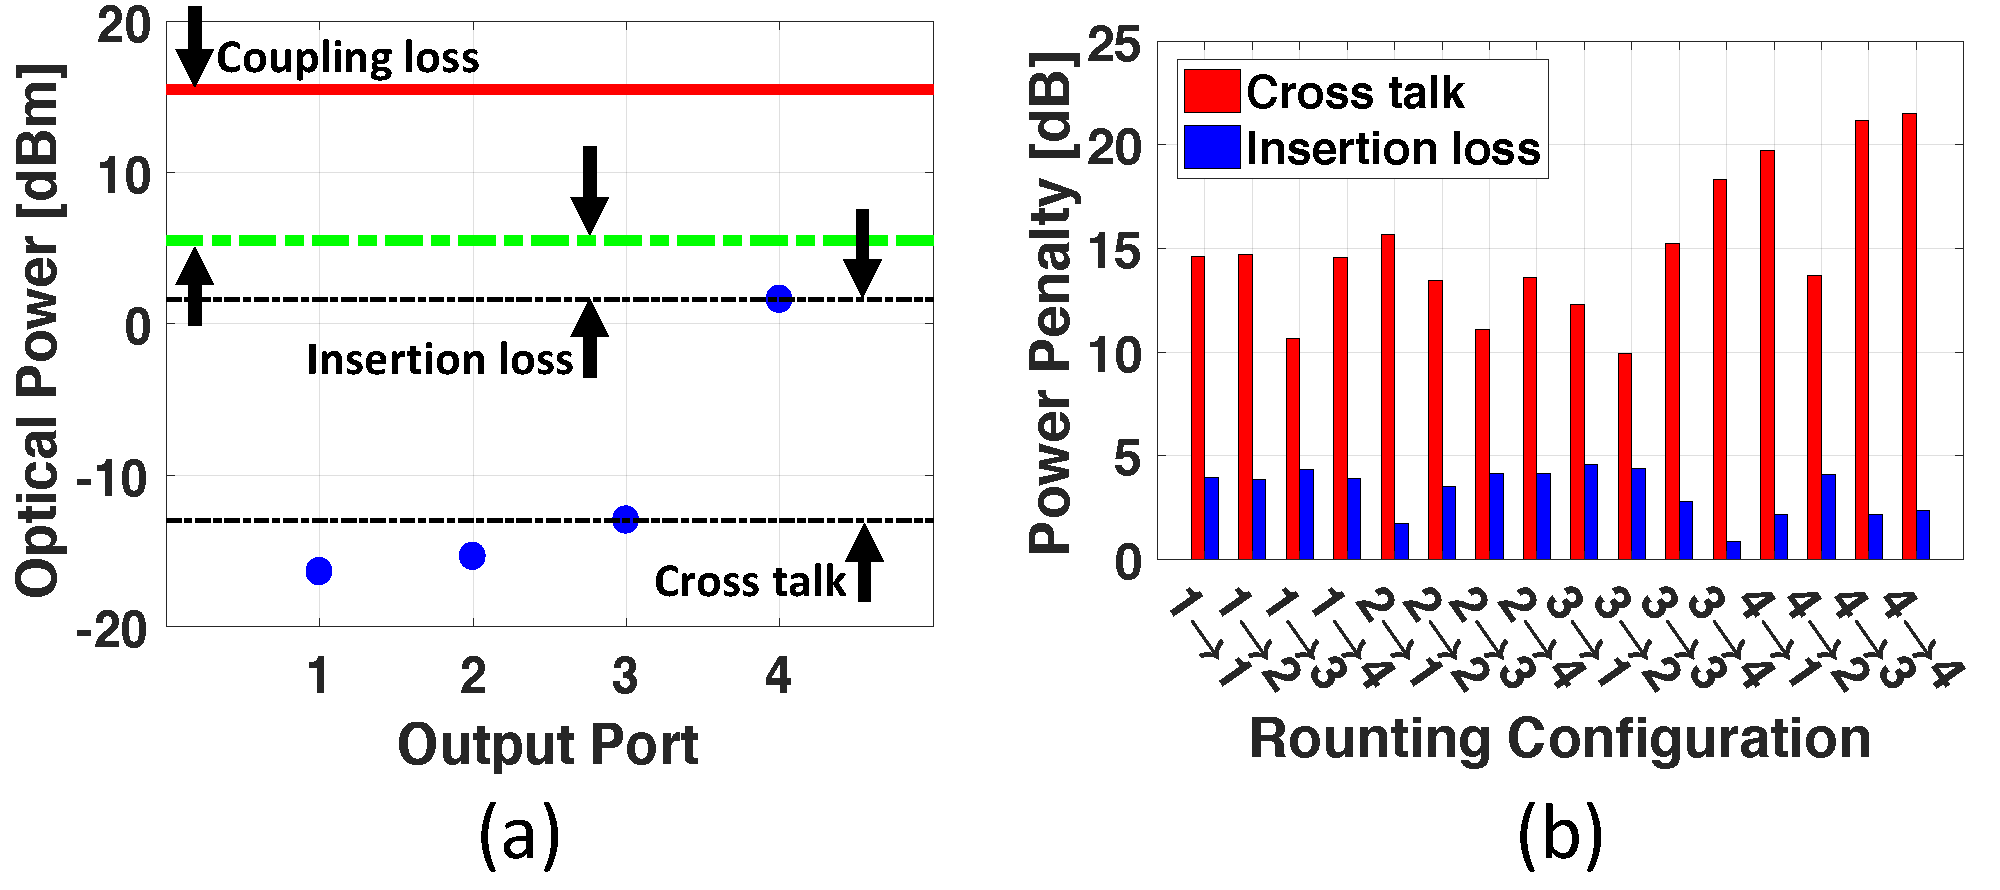
\includegraphics[width=13cm]{Chapter5/fig8_ER_IL3}
\caption{(a) Received optical power measured at all output ports for a single configuration of the switch: input optical data from port 1 to output port 4 (1$\rightarrow$4). The red horizontal line represents the input optical power. The difference to the dashed green line is the loss due to optical fiber coupling. The differences between the green and top dashed black is the insertion loss of switch the and the differences between the top two received optical power represent the cross talk of the configuration. (b) Measured cross talk and insertion loss of all routing configurations of the switch. The x-axis represent the ``input port''$\rightarrow$``output port''.}
\end{figure}

Figure 7(a) shows the measured results for a single routing: 1$\rightarrow$4. Based on the look-up table MZI1-6 are set for the following states [C,-,C,-,B]. The red horizontal line at 15dBm represents the optical input signal operating at 1550nm. 10dB below the laser level, shown in the dashed green line, is the coupling loss. Insertion loss is defined as the loss of the signal due to propagation in the switch in a specific routing configuration. Extinction ratio is the optical power difference between the desired port (port 4) to the second highest level (port 3). For this specific routing the insertion loss is 3.8dB, and the extinction ratio is 14.6dB. 

Similar computations are carried out on the rest of the routing configurations and the results are shown in the bar chart of Fig. 7(b). The crosstalk ranges from 9.92 to 21.51dB and the insertion loss between 0.88--4.59dB. We believe that the variations between the routing performances is caused due to loss variations in the switch such as the couplers and doping level of the heaters. Additionally, due to the small footprint of the $4\times4$ switch (\SI{2000x500 }{\micro\metre}) with vertical and horizontal separation of \SI{250}{\micro\metre} between the $2\times2$ elements, our switch experiences internal thermal crosstalk between the doped-phase shifters when bias voltages are applied simultaneously to the multiple MZIs. 

\subsection{Data transmission}

12.5Gbaud PAM-4 (25Gbps) optical data is used to evaluate the system under transmission conditions, specifically when switching between the routing configurations based on Table 2. Four-level PAM signals, 2$^{15}$ symbols in length, and each containing a training sequence (TS), are generated and loaded into the AWG which was set to operate continuously. After photo-detection at the receive side, the electrical PAM signals are then captured digitally using the RTS. The TS is used both for receiver synchronization and to aid the digital equalization (EQ) process. A Finite Impulse Response (FIR) EQ was used with filter tap weights updated using a decision directed least mean square (DD-LMS) algorithm. EQ, eye-diagram plotting and BER calculations (after PAM demodulation) were performed off-line.

Figure 8(a) shows the collected (oversampled) eye diagrams from the output ports for the 1$\rightarrow$4 routing. The results align with the power levels measured in Fig. 7a. As expected, an open eye is observed at port 4 with a calculated BER of 3.6$\times 10^{-4}$. The next highest optical power is observed in port 3, compared to port 1 and 2, this corresponds to the V{\scriptsize{p-p}} of the measured eyes diagrams. Figure 8(b) summarizes the calculated BERs at the designated output port based on the PC calibrated routing configuration. All the routings exhibit BER performance between 2.7$\times 10^{-4}$ to 5.9$\times 10^{-4}$, which is lower than 7\% overhead hard-decision FEC limit (BER<3.8$\times 10^{-3}$).

\begin{figure}[h!]
\centering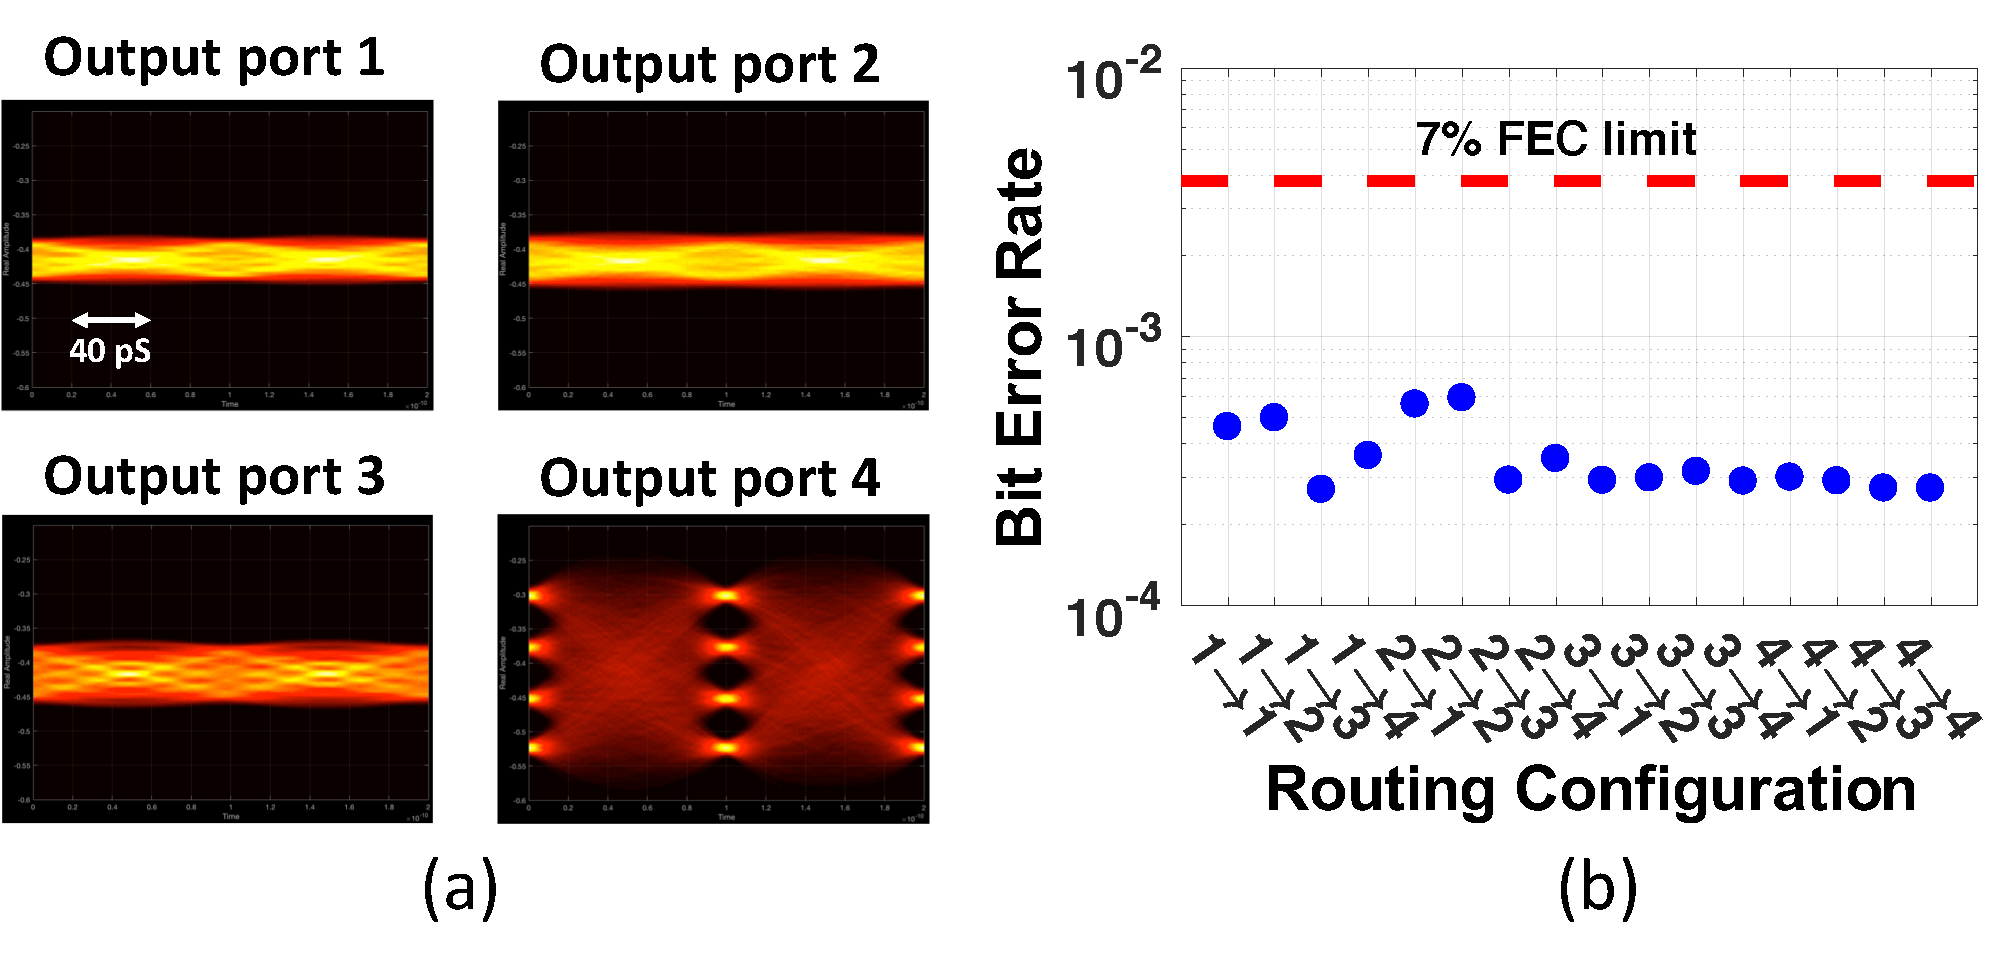
\includegraphics[width=13.5cm]{Chapter5/fig9_eye2}
\caption{Eye diagram results collected at the output ports for a single configuration of the switch: input optical data from port 1 to output port 4 (1$\rightarrow$4). (b) BER results of PAM 25Gbps for all possible routing configurations of the switch. The x-axis represent the ``input port"$\rightarrow$ ``output port".}
\end{figure} 



\section{Conclusion}
%After proofreading the manuscript, compress your .TEX manuscript file and all figures (which should be in EPS format, or PDF format if you are using PDF-\LaTeX) in a ZIP, TAR or TAR-GZIP package. Prism, OSA's article tracking system, will process in \LaTeX mode by default but will use PDF-\LaTeX if PDF figure files are detected. Note: TAR or TAR-GZIP is no longer required. All files must be referenced at the root level (e.g., file \texttt{figure-1.eps}, not \texttt{/myfigs/figure-1.eps}). If there is video or other supplementary materials, the associated files should be uploaded separately.

The use of the PC effect is demonstrated as a topology agnostic solution for calibrating MZI based silicon photonic switches. The steady state and the transient time response is experimentally characterized and analytical models PC current are presented. Based on the effect, a general calibration algorithm that supports cascaded MZI switch designs is outlined. 

The calibration procedure is carried out on a 4$\times$4 Benes design and verified against a more standard procedure using external PD, and is found to operate within a few percent of difference. The calibrated control biases for the cross and bar states are used to reconfigure the switch system for all possible input to output routings. Each configuration is experimentally evaluated for insertion loss (0.88--4.59dB), cross talk (9.92--21.51dB) and BER of 25Gbps PAM4 signals (2.7$\times 10^{-4}$--5.9$\times 10^{-4}$). 

The results prove that the doped phase-shifter heaters can be utilized for both controlling the state of a 2$\times$2 element and as a fast monitoring element of the optical power levels. This provides advantages in terms of saving switch footprint area, reducing design complexity and lower I/O pin count which are important metrics in the design and deployment of scalable photonic switches.